% Chapter 1

\chapter{Introducción general} % Main chapter title

\label{Chapter1} % For referencing the chapter elsewhere, use \ref{Chapter1} 
\label{IntroGeneral}

A continuación, se presentan los lineamientos básicos en cuanto al funcionamiento de la Central Nuclear Atucha II, el diseño termohidráulico de la misma, y los métodos de cálculo de Potencia Límite de Canal y estimación de Flujo Crítico de Calor.

\section{Contexto y motivación}
Uno de los cálculos más importantes en el diseño termohidráulico de un reactor PHWR (del inglés, \textit{Pressurized Heavy Water Reactor}) es el de las Potencias Límite de Canal (PLC). Este cálculo puede necesitar repetirse más de un millón de veces durante cada iteración del cálculo de una estrategia de recambio de combustibles, lo que implica un alto costo computacional. Por lo tanto, obtener una herramienta que permita computar de manera eficiente las PLC e identificar los casos más críticos a ser evaluados con los códigos termohidráulicos, es de alto interés.

Adicionalmente, en el cálculo con los códigos termohidráulicos, un paso fundamental es la estimación del Flujo Crítico de Calor (CHF, del inglés \textit{Critical Heat Flux}) en función de las condiciones locales del fluido. Hoy en día, esto se realiza con métodos que se dividen en dos: fórmulas semi-empíricas que buscan capturar la alta dimensionalidad del problema, y tablas de Flujo Crítico de Calor obtenidas de ensayos en geometrías simples que luego son modificadas por factores ad-hoc para replicar lo mejor posible los ensayos realizados sobre las geometrías reales del canal refrigerante del reactor.

\section{Central Nuclear Atucha II}
La Central Nuclear Atucha II (CNA-UII) se ubica en la localidad de Lima, en la provincia de Buenos Aires, Argentina. Es una central nuclear de tipo PHWR, que utiliza agua pesada (óxido de deuterio) como moderador y refrigerante, y uranio natural como combustible. El reactor nuclear genera 2175 MW térmicos, proveyendo 745 MW eléctricos al Sistema Argentino de Interconexión (SADI). En la Figura \ref{fig:cna2} se aprecia una foto aérea de la central.

La CNA-UII comenzó su construcción en 1982, pero debido a diversos factores fue suspendida en 1994. En 2006, la empresa Nucleoeléctrica Argentina S.A. (NASA) retomó la construcción de la central, logrando su primer criticidad el 3 de junio de 2014, y finalmente obteniendo en 2016 su licencia de operación comercial. El diseño de la CNA-UII es similar al de la Central Nuclear Atucha I (CNA-UI), emplazada en el mismo predio, desarrollado originalmente por la empresa alemana Siemens-KWU.

\begin{figure}[htbp]
	\centering
	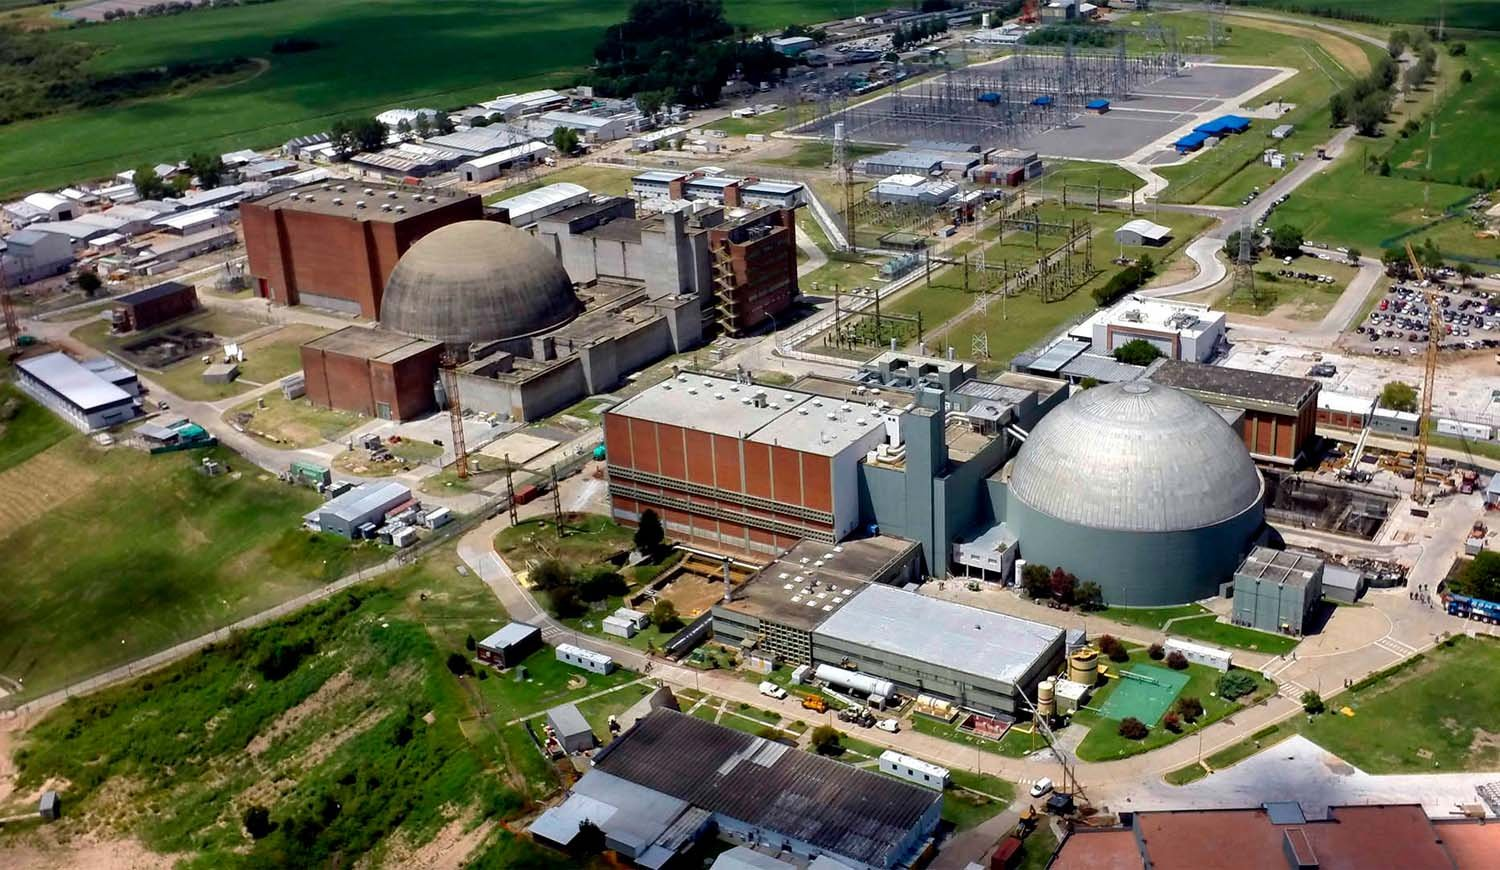
\includegraphics[width=.6\textwidth]{./Figures/cna2_aerea.jpg}
	\caption{Fotografía aérea de la Central Nuclear Atucha II.}
	\label{fig:cna2}
\end{figure}

\section{Diseño Termohidráulico de la Central Nuclear Atucha II}
El diseño termohidráulico de la CNA-UII tiene por objetivo "proporcionar una adecuada transferencia de calor compatible con la tasa de generación de calor en el núcleo y, con la capacidad de remover calor del sistema refrigerante del reactor. Además de los datos principales para el sistema refrigerante del reactor (geometría, caudal másico, nivel de presión y temperatura), el diseño termohidráulico especifica la configuración para los sistemas de control, limitación y protección del reactor que aseguran una operación segura de la planta dentro de los límites aceptables", según lo establecido en el Informe Final de Seguridad (IFS) de la CNA-UII \citep{IFS_CNA2}.

En la Tabla \ref{tab:condiciones_operacion_cna2} se presentan los principales parámetros de diseño y condiciones de operación de la CNA-UII. Se tiene un reactor con 451 elementos combustibles, cada uno alojado en un canal refrigerante, el cual toma agua pesada del plenum inferior, la calienta removiendo calor de los combustibles, y la retorna al circuito primario en el plenum superior. El núcleo se encuentra dividido en 5 zonas hidráulicas, cada una con un caudal másico característico, dado por un restrictor de caudal distintivo para cada zona de 1 a 4. La zona 5 no tiene restricción de caudal. Esta división en zonas hidráulicas se realizó con el criterio de obtener un salto entálpico uniforme en el núcleo, por lo que las zonas periféricas con menor potencia reciben menor caudal. En la Figura \ref{fig:zonas_hidraulicas} se presenta una imagen esquemática de la distribución de los canales en el núcleo de la CNA-UII, y las zonas hidráulicas del mismo.

\begin{table}[h]
	\centering
	\caption{Principales parámetros de diseño y condiciones de operación de la Central Nuclear Atucha II. \citep{IFS_CNA2}}
	\begin{tabular}{l c}    
        \toprule
        \textbf{Condiciones Generales de Operación} & \textbf{CNA-UII} \\
        \hline
        Potencia térmica del reactor & 2160 $\text{MW}_\text{th}$ \\
        Caudal másico total & 10576 $\nicefrac{\text{kg}}{\text{s}}$ \\
        Presión del Sistema Primario & 115 bar \\
        Temperatura de entrada del refrigerante & 277.8 $\degree\text{C}$ \\
        Temperatura de salida del refrigerante & 314.6 $\degree\text{C}$ \\
        Cantidad de zonas hidráulicas del núcleo & 5 \\
        Cantidad de elementos combustibles en el núcleo & 451 \\
        Cantidad de barras combustibles por elemento combustible & 37 \\
		\bottomrule
		% \hline
	\end{tabular}
	\label{tab:condiciones_operacion_cna2}
\end{table}

\begin{figure}[htbp]
	\centering
	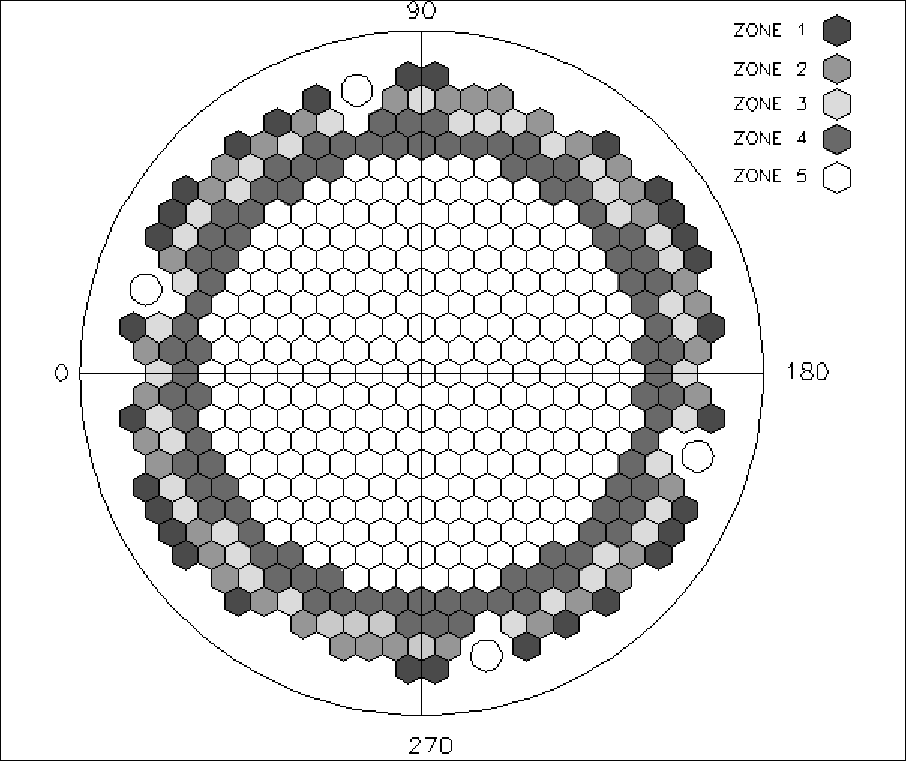
\includegraphics[width=.6\textwidth]{./Figures/zonas_hidraulicas.png}
	\caption{Esquematización de los canales refrigerantes en el núcleo de la CNA-UII y las 5 zonas hidráulicas. \citep{IFS_CNA2}}
	\label{fig:zonas_hidraulicas}
\end{figure}

Para cumplir con los criterios de diseño y operación segura establecidos en el IFS, se deben cumplir dos principales criterios en cuanto a la potencia a la que pueden operar los combustibles dentro del núcleo: el criterio de límite de vacío a la salida de los canales refrigerantes y el criterio de Apartamiento de la Ebullición Nucleada (DNB, del inglés \textit{Departure from Nucleate Boiling}).

En primer lugar, la fracción de vacío ($\alpha$) se define como el porcentaje del área a la salida del canal ocupada por vapor:
\begin{equation}
    \alpha = \frac{A_\text{vapor}}{A_\text{vapor} + A_\text{líquido}},
\end{equation}
y tiene un límite autoimpuesto para evitar vibraciones excesivas en los elementos combustibles y los componentes que aseguran su rigidez estructural. La fracción de vacío está relacionada con el título termodinámico ($x$) de la mezcla de vapor y líquido por la siguiente ecuación:
\begin{equation}
    \alpha = \cfrac{1}{1 + \cfrac{1-x}{x}\cdot \cfrac{\rho_v}{\rho_l}\cdot S},
\end{equation}
siendo $S$ el \textit{slip ratio}, definido como el cociente entre la velocidad del vapor y la velocidad del líquido:
\begin{equation}
    S = \frac{v_v}{v_l}.
\end{equation}

El límite por DNB se explica en la siguiente sección.

\section{Apartamiento de la Ebullición Nucleada (DNB)}

Para poder explicar el fenómeno de DNB, primero se debe introducir el régimen de flujo típico de un reactor de tipo PHWR. En este tipo de reactores el fluido refrigerante se encuentra subenfriado a la entrada del canal refrigerante, y a medida que asciende por el mismo puede transicionar a un régimen de ebullición nucleada, donde se forman burbujas de vapor en la superficie de las vainas combustibles. 

La ebullición nucleada es un régimen de transferencia de calor muy eficiente, ya que las burbujas que se forman en la superficie facilitan la transferencia de calor al líquido. En la Figura \ref{fig:nukiyama} se puede observar la curva de Nukiyama \citep{NUKIYAMA1966}, que representa la relación entre el flujo de calor y la diferencia entre la temperatura de pared y la temperatura de saturación del líquido, para el caso de un cable sumergido en una pileta de agua. Se observa que hasta el comienzo de la ebullición nucleada (ONB, del inglés \textit{Onset of Nucleate Boiling}), el flujo aumenta con la diferencia de temperatura. Luego del ONB, la pendiente se incrementa, es decir, que aumenta la capacidad de transferencia de calor. Sin embargo, este incremento tiene un límite, el punto B de la curva o CHF. En ese punto se tiene un salto repentino al punto D, donde la temperatura de pared aumenta drásticamente, entrando en un régimen de ebullición por película, donde la transferencia de calor es muy ineficiente por la película de vapor que aisla la pared calefaccionada del líquido.

En la Figura \ref{fig:dnb} se tiene el mismo fenómeno, pero representado en un tubo cuyas paredes están calefaccionadas, al cual ingresa líquido por la parte inferior. Se observa que al ascender el régimen pasa de transferencia por convección al líquido subenfriado, a ebullición subenfriada (es decir, con temperatura promedio del líquido por debajo de la temperatura de saturación), a ebullición nucleada en saturación, y finalmente al apartamiento de la ebullición nucleada y la ebullición en película.

El criterio de seguridad del diseño termohidráulico de una central es garantizar la integridad las vainas combustibles y las pastillas de combustible dentro de las mismas. Para esto, se requiere que la temperatura de las mismas esté por debajo de un cierto valor establecido en el diseño. Si retornamos a la curva de Nukiyama (Figura \ref{fig:nukiyama}), podemos comprender que evitar el DNB es entonces un principio fundamental en el diseño termohidráulico de un reactor PHWR. 

\begin{figure}[htbp]
	\centering
	% 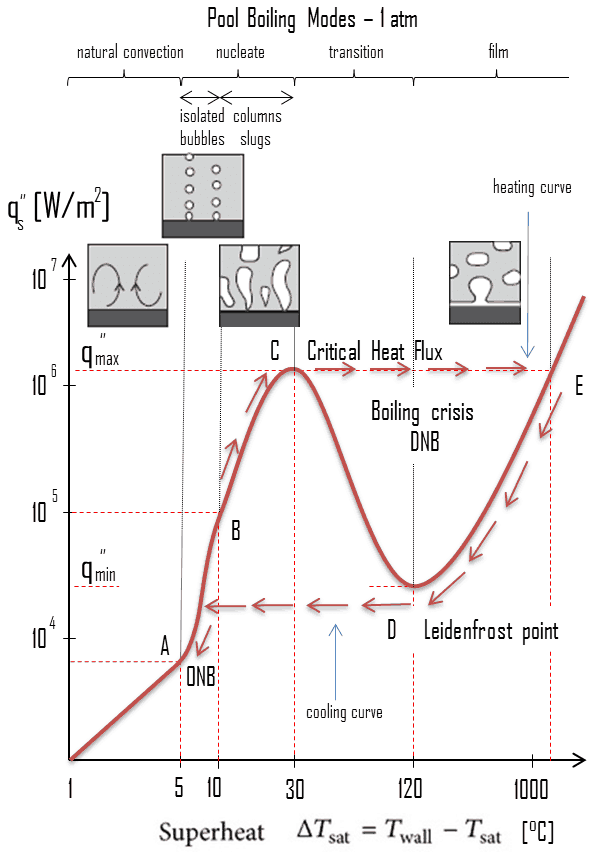
\includegraphics[width=.6\textwidth]{./Figures/curva_nukiyama.png}
	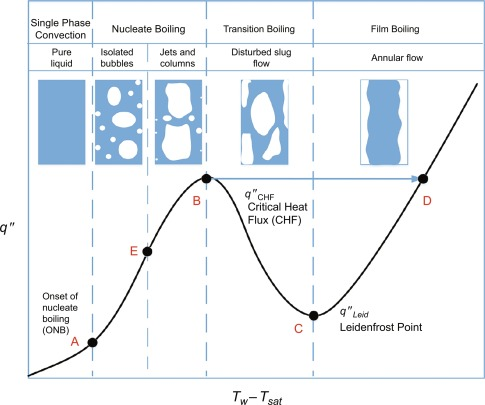
\includegraphics[width=.8\textwidth]{./Figures/nukiyama.jpg}
	\caption{Curva de Nukiyama.}
	\label{fig:nukiyama}
\end{figure}

\begin{figure}[htbp]
	\centering
	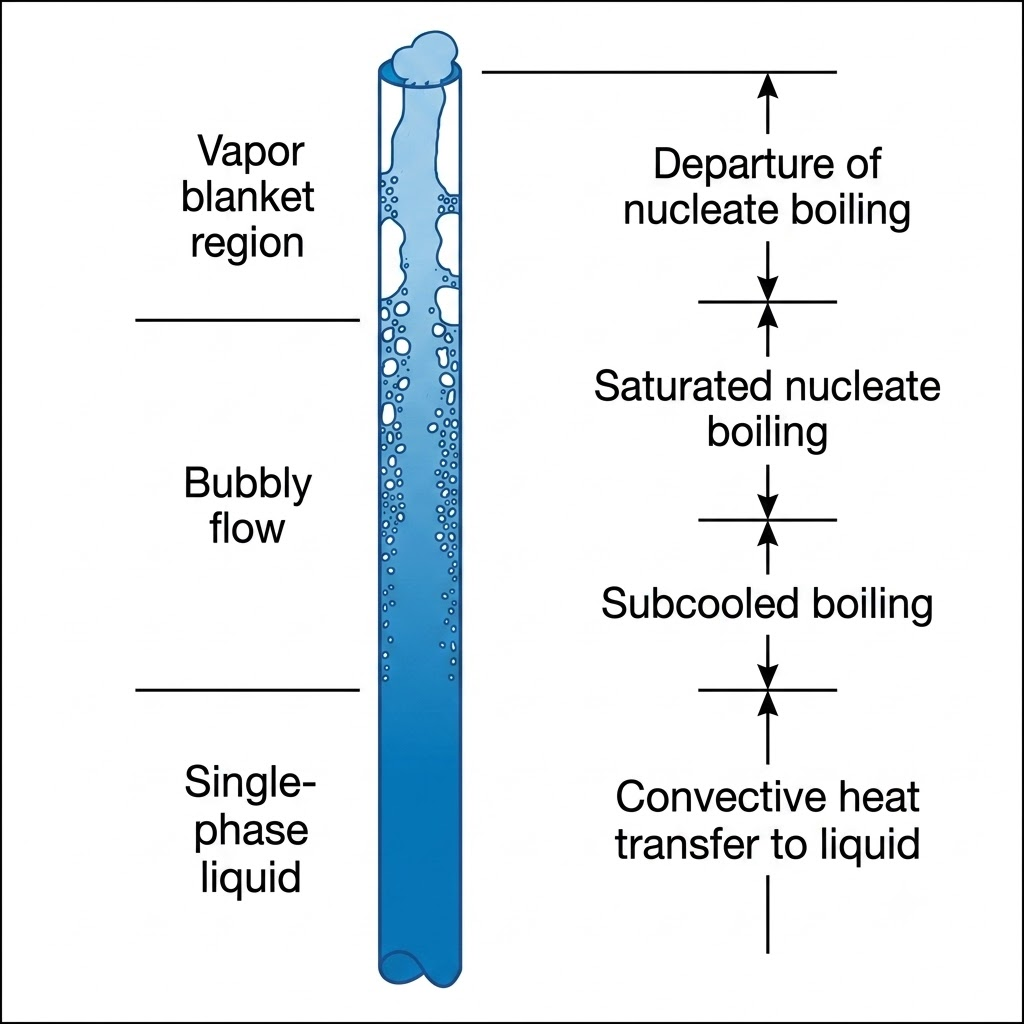
\includegraphics[width=.7\textwidth]{./Figures/dnb.jpg}
	\caption{Esquematización del Apartamiento de la Ebullición Nucleada (DNB) en un tubo.}
	\label{fig:dnb}
\end{figure}

\section{Cálculo de Potencia Límite de Canal}
Se tiene entonces dos límites relacionados a la potencia a la que puede operar un canal refrigerante: por fracción de vacío y por DNB. El cálculo de la Potencia Límite de Canal (PLC) consiste en determinar la potencia máxima a la que puede operar un canal refrigerante sin superar los límites de fracción de vacío y DNB.

Para tener en cuenta la incerteza en la estimación del CHF, la sensibilidad de ésta con respecto a las condiciones de operación del núcleo, y que todos los transitorios operacionales previstos deben cumplir con asegurar que no se tenga DNB, se debe plantea asegurar un márgen al DNB o DNBR (del inglés, \textit{Departure from Nucleate Boiling Ratio}). Entonces, la PLC por DNB en rigor es aquela potencia a la cual se mantiene el DNBR establecido en el IFS de la CNA-UII, el cual es característico para cada zona hidráulica.

El cálculo de las PLC para la CNA-UII se realiza utilizando dos códigos termohidráulicos. En primer lugar se utiliza el código COBRA3-CP \citep{cobra3cp}, un código de subcanales desarrollado originalmente por el MIT, modificado posteriormente por la empresa alemana Siemens-KWU en los años ochenta, y luego por INVAP en el año 2008. Estas modificaciones han permitido adaptar el código, pensado originalmente para reactores de tipo PWR, a la geometría específica del reactor de la CNA-UII. El código COBRA-3CP permite simular el comportamiento termohidráulico de un canal refrigerante, y determinar la potencia a la que se alcanza el límite por vacío y el límite por DNB.

Por otro lado, el código AXCNA \citep{axcna}, de desarrollo interno de la Gerencia de Análisis de Seguridad y Diseño del Núcleo (GASyDN) de NASA, permite simular el comportamiento hidráulico de todo el sistema primario para obtener la pérdida de carga en el reactor, a partir de la señal de salto de presión en las bombas del primario. Luego, se utiliza este valor para calcular la distribución de caudal entre los canales refrigerantes, en función de los restrictores de caudal y las pérdidas hidráulicas por la generación de vapor en los canales. Esto permite estimar en tiempo real el límite al DNB de cada canal refrigerante, y, en conjunto con los medidores de potencia in-core, provee al sistema de limitación de potencia (RELEB, del alemán \textit{Reaktor LeistungsBegrenzung}) la información necesaria para computar el márgen de potencia en tiempo real.

Las PLC también son utilizadas para el cómputo de las estrategias de recambios de combustibles, teniendo un proceso iterativo entre el cómputo neutrónico de las estrategias y el recálculo termohidráulico de las PLC. Por lo tanto, es de interés tener un método rápido y confiable para evaluar las estrategias de recambio, e identificar los estados del reactor más comprometido dentro de las mismas para su análisis detallado con AXCNA y COBRA3-CP.

\subsection{Códigos de subcanales}
A continuación se desarrolla la teoría base del método de los códigos de subcanales, utilizando como base el Manual de Modelos de COBRA3-CP \citep{cobra3cp}.

En la Figura \ref{fig:sch} se esquematiza la discretización en subcanales. Esta busca generar elementos prismáticos, los cuales tienen algunas caras en contacto con las vainas combustibles, y otras en contacto con subcanales adyacentes. De esta forma, se puede resolver por medio de las ecuaciones de conservación en su formato unidimensional, y sólo es necesario agregar una componente transversal debido a la comunicación entre subcanales y una ecuación de conservación para la cantidad de movimiento transversal.

\begin{figure}[htbp]
	\centering
	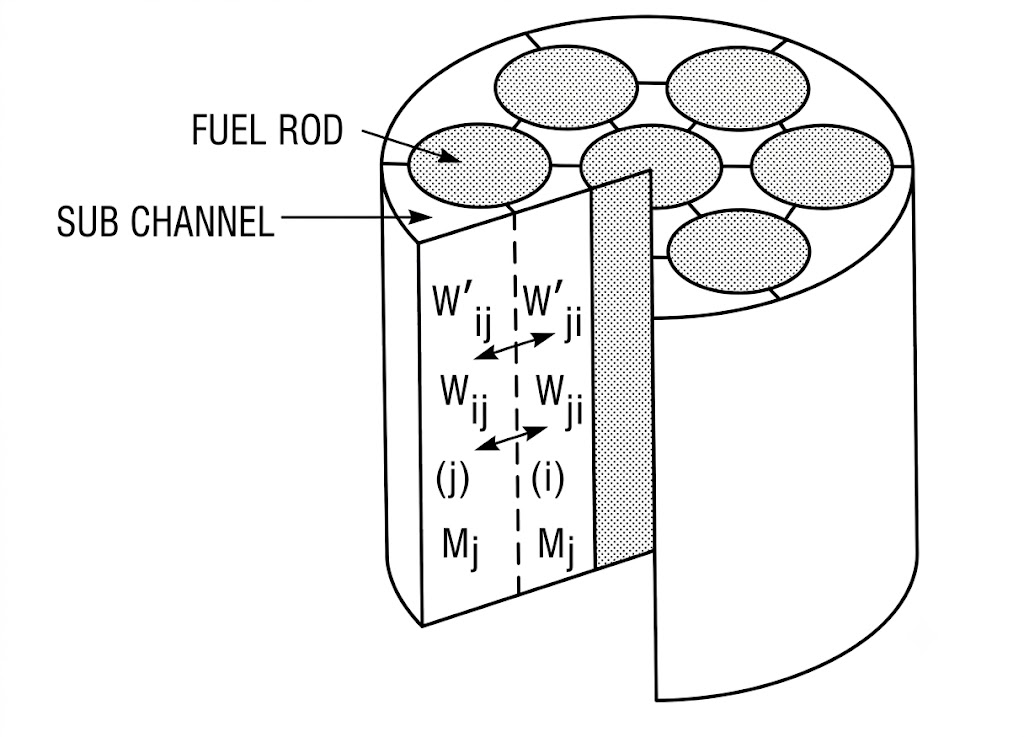
\includegraphics[width=.6\textwidth]{./Figures/subchannels.jpg}
	\caption{Esquematización de discretización en subcanales. Obtenido del Manual de Modelos de COBRA3-CP \citep{cobra3cp}}
	\label{fig:sch}
\end{figure}

Entonces se desarrollan las ecuaciones de conservación para un dado subcanal $i$ a continuación. En primer lugar, la conservación de la masa viene dada por:

\begin{equation}
    A \frac{\partial \rho_i}{\partial t} + \frac{\partial \dot{m}_i}{\partial z} + \sum_j w_{ij} = 0,
\end{equation}
siendo $A$ el área de paso, $\rho$ la densidad, $\dot{m}$ el caudal másico, $z$ la coordenada axial y $w_{ij}$ el factor de flujo cruzado por diversión.

Luego, se presenta la conservación de la energía:
\begin{equation}
    A \frac{\partial (\rho h)_i}{\partial t} + \frac{\partial (\dot{m} h)_i}{\partial z} = q'_i - \sum_j w^{*H}_{ij} (h_i - h_j) - \sum_j w_{ij} h^* + A \frac{Dp}{Dt},
\end{equation}
siendo $h$ la entalpía, $q'$ el flujo de calor, $w^{*H}_{ij}$ el factor de flujo cruzado efectivo por transporte de energía, $h^*$ la entalpía transportada por diversión y $p$ la presión.

En tercer lugar, se tiene la conservación de la cantidad de movimiento axial:
\begin{equation}
    \frac{\partial \dot{m}_i}{\partial t} + \sum_j w_{ij} u^*_j + \frac{\partial (\dot{m} u_z)_i}{\partial z} = -A \rho g_z - A \frac{\partial p}{\partial z} - \sum_j w^{*M}_{ij} (u_{zi} - u_{zj}) - F_{iz},
\end{equation}
siendo $u^*$ la velocidad axial transportada por diversión, $u$ la velocidad con subíndice según la dirección, $g_z$ la aceleración de la gravedad, $w^{*M}_{ij}$ el factor de flujo cruzado efectivo por transporte de momento y $F_i$ la fuerza de arrastre por fricción y forma con subíndice según la dirección.

Por último, la conservación de la cantidad de movimiento transversal viene dada por:
\begin{equation}
    \frac{\partial w_{ij}}{\partial t} + \frac{\partial w_{ij} u_x}{\partial x} + \frac{\partial w_{ij} u_z}{\partial x} = - s_{ij} \frac{\partial p}{\partial x} - F_{ix}.
\end{equation}

Es importante notar que los términos de flujo cruzado son de carácter empírico, y para su determinación se utilizan ensayos de mezclado en condiciones subenfriadas para la geometría específica que se quiere modelar. Estos términos han sido determinados de esta forma para el \textit{bundle} de la CNA-UII, y se continúan proponiendo mejoras para su modelado.